%2multibyte Version: 5.50.0.2953 CodePage: 1252
% green
% blue
% orange
% purple
% red
% resets numbering each section

\ifdefined\extendedversion\else
  \PassOptionsToClass{handout}{beamer}
\fi
\documentclass[xcolor=x11names,compress,aspectratio=169]{beamer}%
\usepackage{amsmath}
\usepackage{amsfonts}
\usepackage{amssymb}
\usepackage{graphicx}
\usepackage{tikz}
\usepackage{dcolumn}
\usepackage{tikz}%
\setcounter{MaxMatrixCols}{30}
%TCIDATA{OutputFilter=latex2.dll}
%TCIDATA{Version=5.50.0.2953}
%TCIDATA{Codepage=1252}
%TCIDATA{CSTFile=beamer.cst}
%TCIDATA{Created=Monday, May 13, 2013 15:44:12}
%TCIDATA{LastRevised=Monday, November 24, 2025 12:02:19}
%TCIDATA{<META NAME="GraphicsSave" CONTENT="32">}
%TCIDATA{<META NAME="SaveForMode" CONTENT="1">}
%TCIDATA{BibliographyScheme=Manual}
%TCIDATA{<META NAME="DocumentShell" CONTENT="Other Documents\SW\Slides - Beamer">}
%TCIDATA{Language=American English}
%BeginMSIPreambleData
\providecommand{\U}[1]{\protect\rule{.1in}{.1in}}
%EndMSIPreambleData
%\usepackage{etex} %vers l'infini et au-dela
\usepackage{minted}
\beamertemplatenavigationsymbolsempty
\usepackage[utf8]{inputenc} 
\usepackage[T1]{fontenc} % pour taper les lettres accentuees
%\usepackage[francais, english]{babel} %le rapport est en franÁais 
\usepackage{amsthm,amssymb,amsbsy,amsmath,amsfonts,amscd,mathrsfs}
\usepackage{geometry} %pour la modification des marges
%\usepackage{fancyhdr} %pour modification des pieds de page
%\usepackage{lastpage} %numero de la derniËre page
\usepackage{lmodern}
\usepackage{lscape} % Pour pouvoir activer le mode landscape
\usepackage{booktabs} %tableaux
\usepackage{float}	%pour forcer le placement des images.
\usepackage{graphicx} %pour afficher des images
\usepackage{longtable} %tables sur plusieurs pages
\usepackage{animate} %transformer des gifs
\usepackage{caption}
\captionsetup{labelformat=simple}
\setbeamertemplate{caption}[numbered]
\setbeamerfont{caption}{size=\scriptsize}
\usepackage[scriptsize]{subfigure}
\usepackage{multirow} 			%fusionner lignes
\usepackage{tikz}
\usepackage{adjustbox}
\usetikzlibrary{arrows,positioning}
\usetikzlibrary{mindmap,trees,shadows,backgrounds}
\usepackage{tabularx}
\usepackage{verbatim}%insertion de code
\usepackage{listings}
\usepackage{dsfont} % Pour les lettres mathematiques
\usepackage{hyperref} %pour que les references soient des liens hypertextes
\usepackage{natbib}
\usepackage{bibentry}
\usepackage{color}
\definecolor{bg}{rgb}{0.95,0.95,0.95}

\def\LECTURENAME{Mod\'elisation, estimation, simulation des risques climatiques}
\def\DIPLOMA{Master in Economics, 2$^{nd}$ year}
\def\UNIV{Ecole Polytechnique}
\def\WEBPAGE{\href{http://vermandel.fr/btm/}{http://vermandel.fr/btm}}
\def\SHORTNAME{Modélisation, estimation, simulation des risques climatiques}



%\usepackage{mathpazo}
\usepackage{multimedia}
\usepackage{dcolumn}
\usepackage{mathtools}
\usepackage{xspace}
\usepackage{array}%

\usepackage{graphicx}

\definecolor{light-gray}{gray}{0.85}
\usepackage{ragged2e} % Pour justifier
\definecolor{bleu}{RGB}{0,129,188}
\definecolor{rouge}{RGB}{238,50,78}
\definecolor{orange}{RGB}{255,100,0}
\definecolor{vert}{RGB}{0,157,87}
\newtheorem{hypothese}{Hypoth\`ese}
\newtheorem{remarque}{Hypoth\`ese}
\newtheorem{theoreme}{Th\'eor\`eme}[section]
\newtheorem{definitionDeux}{D\'efinition}[section]
\newcommand{\iid}{\stackrel{\mathrm{iid}}{\sim}}
\usepackage[official,right]{eurosym} % symbols euro
\usepackage{gensymb} % symbole degre \degre
\usepackage{eurosym} % symbole euro
\usepackage{rotating}
\usepackage{multicol}

% Bibliographie
%\usepackage{bib entry}
%\nobibliography*
%\let\newblock\relax

%\usepackage[notocbib]{apacite}
%\usepackage[style=apa]{biblatex}
%\usepackage[round]{natbib}
%\usepackage[style=authoryear]{biblatex}
%\usepackage[backend=bibtex, style=authoryear-comp]{biblatex}
%\usepackage{biblatex}
%\renewcommand*{\bibfont}{\scriptsize} % Pour avoir la biblio en plus petit
%\usepackage{apacite}
%\bibliographystyle{apacite}

\justifying %on justifie le texte du document
\definecolor{deepblue}{RGB}{0,129,188}
\definecolor{deepblue2}{RGB}{158, 64, 57}
\definecolor{deepblue3}{RGB}{245, 84, 66}


% Pour l'annexe (http://tex.stackexchange.com/questions/2541/beamer-frame-numbering-in-appendix)
\newcommand{\backupbegin}{
   \newcounter{framenumberappendix}
   \setcounter{framenumberappendix}{\value{framenumber}}
}
\newcommand{\backupend}{
   \addtocounter{framenumberappendix}{-\value{framenumber}}
   \addtocounter{framenumber}{\value{framenumberappendix}} 
}

%\usepackage{epstopdf}
%\epstopdfDeclareGraphicsRule{.gif}{png}{.png}{%
%  convert gif:#1 png:\OutputFile
%}
%\AppendGraphicsExtensions{.gif}

% A NE PAS UTILISER !
%\let\olditem=\item% 
%\renewcommand{\item}{\olditem \justifying}%

\justifying

%\graphicspath{{../images}}


\usepackage{dcolumn}


% THEME %
\usetheme{Frankfurt}
\useoutertheme[subsection=false,shadow]{miniframes}

\addtobeamertemplate{background canvas}{\transfade[duration=.3]}{}

% Fonts
%\usefonttheme[onlymath]{serif}
%\usefonttheme{structuresmallcapsserif}
%\usefonttheme[onlymath]{mathserif}
%\usefonttheme{serif}
\setbeamerfont{section in head/foot}{size=\tiny, shape=\normalfont}
\setbeamerfont{subsection in toc}{shape=\normalfont, size = \scriptsize}
\setbeamerfont{section in toc}{size = \small, shape=\normalfont}
% Colours
\setbeamercolor{section in head/foot}{fg=black, bg=gray!5}
\setbeamercolor{frametitle}{bg=white, fg=black}
\setbeamercolor{lower separation line head}{bg=black!5}

\setbeamertemplate{sections/subsections in toc}[square]
\setbeamertemplate{items}[triangle]
\setbeamertemplate{itemize subitem}[triangle]
\setbeamertemplate{itemize subsubitem}[ball]
\setbeamertemplate{enumerate items}[default]
\setbeamertemplate{frametitle}[default][rounded=false,shadow=true]

\setbeamercovered{transparent}



\usepackage{assets/beamerouterthemeEwen}
\usepackage{assets/beamercolorthemeEwen}
\usepackage{assets/beamerhighlight}


\newcommand*\grasO[1]{\textbf{\textcolor{orange}{#1}}} 
\newcommand*\grasR[1]{\textbf{\textcolor{rouge}{#1}}}
\newcommand*\grasV[1]{\textbf{\textcolor{vert}{#1}}} 
\newcommand*\grasB[1]{\textbf{\textcolor{bleu}{#1}}} 


\definecolor{rcp26}{RGB}{39, 55, 122}
\definecolor{rcp45}{RGB}{112, 159, 200}
\definecolor{rcp60}{RGB}{222, 99, 43}
\definecolor{rcp85}{RGB}{205, 16, 32}
\definecolor{dp}{RGB}{181, 73, 60}

\newcommand*\grasRCPa[1]{\textbf{\textcolor{rcp26}{#1}}}
\newcommand*\grasRCPb[1]{\textbf{\textcolor{rcp45}{#1}}} 
\newcommand*\grasRCPc[1]{\textbf{\textcolor{rcp60}{#1}}} 
\newcommand*\grasRCPd[1]{\textbf{\textcolor{rcp85}{#1}}} 
%\newcommand {\red} {\color{red}}
\newcommand {\white} {\color{white}}
%\newcommand {\black} {\color{black}}
\def\Frac#1#2{ #1 \color{red}\above 0.4pt \normalcolor #2}


\usetikzlibrary{decorations}
\usetikzlibrary{decorations.pathmorphing}
\usetikzlibrary{shapes.geometric}
\usetikzlibrary{calc}
\usetikzlibrary{decorations.fractals}
\useoutertheme[subsection=false,shadow]{miniframes}
\useinnertheme{default}
\usefonttheme{serif}
\setbeamerfont{title like}{shape=\scshape}
\setbeamerfont{frametitle}{shape=\scshape}
\setbeamercolor*{lower separation line head}{bg=DeepSkyBlue4}
\setbeamercolor*{normal text}{fg=black,bg=white}
\setbeamercolor*{alerted text}{fg=dp}
\setbeamercolor*{example text}{fg=black}
\setbeamercolor*{structure}{fg=black}
\setbeamercolor*{palette tertiary}{fg=black,bg=black!10}
\setbeamercolor*{palette quaternary}{fg=black,bg=black!10}
\renewcommand{\(}{\begin{columns}}
\renewcommand{\)}{\end{columns}}
\newcommand{\<}[1]{\begin{column}{#1}}
\renewcommand{\>}{\end{column}}
\setbeamertemplate{navigation symbols}{}
\setbeamertemplate{headline}{}
\setbeamertemplate{footline}
{
\leavevmode
\hbox{\begin{beamercolorbox}[wd=1\paperwidth,ht=2.25ex,dp=1ex,center]{title in head/foot}\usebeamerfont{title in head/foot}\hfill\hspace*{12em}\insertshorttitle\hspace*{3em}
\insertframenumber{} / \inserttotalframenumber\hspace*{1ex}
\end{beamercolorbox}}
\vskip0pt
}
\newcommand {\red} {\color{red}}
\newcommand {\black} {\color{black}}
\newcommand{\green}{\color{green}}
\definecolor{deepblue}{RGB}{0,129,188}
\newcommand{\pink}{\color{magenta}}
\newcommand{\blue}{\color{deepblue}}
\hypersetup{
colorlinks = true,citecolor=deepblue3,linkcolor=deepblue2
}
\setbeamercolor{frametitle}{fg=deepblue2,bg=white}
\makeatletter
\AtBeginSection[]
{
\ifnum \value{framenumber}>2
\begin{frame}<beamer>
\frametitle{Plan}
\tableofcontents[currentsection,subsectionstyle=hide]
\end{frame}
\else
\fi
}
\let\oldtextbf\textbf
\renewcommand{\textbf}[1]{\textcolor{dp}{\oldtextbf{#1}}}
\newcommand*\annotatedFigureBoxGOT[2]{\draw[thick,rounded corners,deepblue2] (#1) rectangle (#2);}
\newcommand*\annotatedFigureBoxARR[2]{\draw[->,thick,rounded corners,deepblue2] (#1) -- (#2);}
\newcommand*\annotatedFigureBoxCustom[8]{\draw[#5,thick,rounded corners] (#1) rectangle (#2);\node at (#4) [fill=#6,thick,shape=circle,draw=#7,inner sep=2pt,font=\sffamily,text=#8] {\textbf{#3}};}
\newcommand*\annotatedFigureBox[4]{\annotatedFigureBoxCustom{#1}{#2}{#3}{#4}{deepblue2}{deepblue2}{black}{black}}
\newcommand*\annotatedFigureText[4]{\node[draw=none, anchor=south west, text=#2, inner sep=0, text width=#3\linewidth,font=\sffamily] at (#1){#4};}
\newenvironment {annotatedFigure}[1]{\centering\begin{tikzpicture}
\node[anchor=south west,inner sep=0] (image) at (0,0) { #1};\begin{scope}[x={(image.south east)},y={(image.north west)}]}{\end{scope}\end{tikzpicture}}

\usetikzlibrary{arrows.meta,positioning,overlay-beamer-styles}
\usetheme[numbering=none,progressbar=frametitle]{metropolis}
\setbeamertemplate{footline}{
\hfill\usebeamerfont{page number in head/foot}\insertpagenumber/\insertpresentationendpage\hspace{1em}
}
\usetikzlibrary{arrows.meta, positioning, shapes.misc, fit}
\newenvironment{stepenumerate}{\begin{enumerate}[<+->]}{\end{enumerate}}
\newenvironment{stepitemize}{\begin{itemize}[<+->]}{\end{itemize} }
\newenvironment{stepenumeratewithalert}{\begin{enumerate}[<+-| alert@+>]}{\end{enumerate}}
\newenvironment{stepitemizewithalert}{\begin{itemize}[<+-| alert@+>]}{\end{itemize} }
\newtheorem{assumption}[theorem]{Assumption}
\setlength{\itemsep}{1em}
\definecolor{ssp1}{RGB}{27,158,119}
\definecolor{ssp2}{RGB}{55,126,184}
\definecolor{ssp3}{RGB}{217,95,2}
\definecolor{ssp4}{RGB}{152,78,163}
\definecolor{ssp5}{RGB}{228,26,28}
\definecolor{forc19}{RGB}{255,230,230}
\definecolor{forc26}{RGB}{255,180,180}
\definecolor{forc45}{RGB}{255,120,120}
\definecolor{forc70}{RGB}{220,50,50}
\definecolor{forc85}{RGB}{150,0,0}
\newif\ifshowslide
\showslidefalse
% Compact is the default: each item list is static.
% The extended wrapper turns lists into progressive overlays for lecture delivery.
\ifdefined\extendedversion
  \let\compactitemize\itemize
  \let\endcompactitemize\enditemize
  \renewenvironment{itemize}{\begin{compactitemize}[<+-| alert@+>]}{\end{compactitemize}}
  \renewenvironment{stepitemize}{\begin{compactitemize}[<+->]}{\end{compactitemize}}
  \renewenvironment{stepitemizewithalert}{\begin{compactitemize}[<+-| alert@+>]}{\end{compactitemize}}
\else
  % Static handout: all list content is fully visible, with no animation fade.
  \renewenvironment{stepitemize}{\begin{itemize}}{\end{itemize}}
  \renewenvironment{stepitemizewithalert}{\begin{itemize}}{\end{itemize}}
  \renewenvironment{stepenumerate}{\begin{enumerate}}{\end{enumerate}}
  \renewenvironment{stepenumeratewithalert}{\begin{enumerate}}{\end{enumerate}}
  \setbeamercovered{transparent=100}
\fi
\begin{document}
%
%TCIMACRO{\TeXButton{GG}{\title[\SHORTNAME]{
%\textsc{\footnotesize\SHORTNAME\\ Session 2\\[0.35em] \Large An Introduction to a Climate Model}
%\\
%}
%\author{ Gauthier Vermandel\\
%{\footnotesize Ecole polytechnique}}
%\date{}}}%
%BeginExpansion
\title[\SHORTNAME]{
\textsc{\footnotesize\SHORTNAME\\ Session 2\\[0.35em] \Large An Introduction to a Climate Model}
\\
}
\author{ Gauthier Vermandel\\
{\footnotesize Ecole polytechnique}}
\date{}%
%EndExpansion
%

%TCIMACRO{\TeXButton{BeginFrame}{\begin{frame}}}%
%BeginExpansion
\begin{frame}%
%EndExpansion
%

%TCIMACRO{\TeXButton{\maketitle}{\maketitle}}%
%BeginExpansion
\maketitle
%EndExpansion
%

%TCIMACRO{\TeXButton{Transition: Box Out}{\transboxout}}%
%BeginExpansion
\transboxout
%EndExpansion%
%TCIMACRO{\TeXButton{EndFrame}{\end{frame}}}%
%BeginExpansion
\end{frame}%
%EndExpansion
%

%TCIMACRO{\TeXButton{BeginFrame}{\begin{frame}}}%
%BeginExpansion
\begin{frame}%
%EndExpansion
%

%TCIMACRO{\QTR{frametitle}{Schedule of the day}}%
%BeginExpansion
\frametitle{Schedule of the day}%
%EndExpansion


\textbf{Objectives}

\begin{itemize}
\item Understanding the \textbf{basics} of climate models to predict world temperatures.

\item Simulating climate models on historical data and make some forecasts
conditional on emission scenarios.%
%TCIMACRO{\TeXButton{vspace}{\vspace{1ex}}}%
%BeginExpansion
\vspace{1ex}%
%EndExpansion

\end{itemize}

\textbf{Materials:}

\begin{itemize}
\item \textsf{notebook\_session2.ipynb} \textit{carbon-cycle and temperature dynamics.}

\item \textsf{climate\_model.pdf} \textit{ODEs, initial conditions and discretization.}

\item \textsf{Climate\_Models.py}\textit{ package to simulate reduced form
climate models.}
\end{itemize}

%

%TCIMACRO{\TeXButton{Transition: Box Out}{\transboxout}}%
%BeginExpansion
\transboxout
%EndExpansion%
%TCIMACRO{\TeXButton{EndFrame}{\end{frame}}}%
%BeginExpansion
\end{frame}%
%EndExpansion


\section{Introduction}%

%TCIMACRO{\TeXButton{BeginFrame}{\begin{frame}}}%
%BeginExpansion
\begin{frame}%
%EndExpansion
%

%TCIMACRO{\QTR{frametitle}{Intro: Why should economists care about climate
%science?}}%
%BeginExpansion
\frametitle{Intro: Why should economists care about climate science?}%
%EndExpansion


\begin{itemize}
\item Climate change is driven by physical processes that can be
\textbf{summarized in a simple causal chain}.

\item Integrated Assessment Models (IAMs) like DICE or FAIR rely on this chain.

\item To interpret or extend IAMs, we need to understand the building blocks.
\end{itemize}

\vspace{0.5cm} \begin{block}{The Climate-Economy Chain}
\[
\text{Emissions} \;\;\rightarrow\;\; \text{Concentrations} \;\;\rightarrow\;\;
\text{Radiative Forcing} \;\;\rightarrow\;\; \text{Temperature} \;\;\rightarrow\;\; \text{Impacts}
\]
\end{block}
\vspace{0.3cm}

\begin{itemize}
\item Each arrow corresponds to a physical process.

\item IAMs implement reduced-form versions of these processes.
\end{itemize}

%

%TCIMACRO{\TeXButton{Transition: Box Out}{\transboxout}}%
%BeginExpansion
\transboxout
%EndExpansion%
%TCIMACRO{\TeXButton{EndFrame}{\end{frame}}}%
%BeginExpansion
\end{frame}%
%EndExpansion
%

%TCIMACRO{\TeXButton{BeginFrame}{\begin{frame}}}%
%BeginExpansion
\begin{frame}%
%EndExpansion
%

%TCIMACRO{\QTR{frametitle}{Intro: Climate science is about big models}}%
%BeginExpansion
\frametitle{Intro: Climate science is about big models}%
%EndExpansion


How do climate scientists study the system?

\begin{itemize}
\item \textbf{General Circulation Models (GCMs)} and \textbf{Earth System
Models (ESMs)}:

\begin{itemize}
\item Simulate atmosphere, ocean, cryosphere, land surface, and biogeochemical cycles.

\item Built on physical laws (fluid dynamics, thermodynamics, radiative transfer).

\item Used in IPCC reports for future climate projections.
\end{itemize}

\item Strengths:

\begin{itemize}
\item High fidelity, spatial detail, many processes included.

\item Provide benchmarks for scientific understanding.
\end{itemize}

\item Limitations for Integrated Assessment Modelling:

\begin{itemize}
\item Extremely computationally intensive (supercomputers).

\item Results not easily integrated into optimization or policy models.
\end{itemize}
\end{itemize}

%

%TCIMACRO{\TeXButton{Transition: Box Out}{\transboxout}}%
%BeginExpansion
\transboxout
%EndExpansion%
%TCIMACRO{\TeXButton{EndFrame}{\end{frame}}}%
%BeginExpansion
\end{frame}%
%EndExpansion
%

%TCIMACRO{\TeXButton{IFSHOW}{\ifshowslide}}%
%BeginExpansion
\ifshowslide
%EndExpansion
%

%TCIMACRO{\TeXButton{BeginFrame}{\begin{frame}}}%
%BeginExpansion
\begin{frame}%
%EndExpansion
%

%TCIMACRO{\QTR{frametitle}{Intro: Global Climate / Earth System Models}}%
%BeginExpansion
\frametitle{Intro: Global Climate / Earth System Models}%
%EndExpansion


\begin{itemize}
\item \textbf{CESM} \textit{(Community Earth System Model, NCAR, USA)}

\item \textbf{HadGEM / UKESM} \textit{(Hadley Centre Global Environment Model,
UK Met Office)}

\item \textbf{MPI-ESM} \textit{(Max Planck Institute Earth System Model,
Germany)}

\item \textbf{GFDL-ESM} \textit{(Geophysical Fluid Dynamics Laboratory, NOAA,
USA)}

\item \textbf{IPSL-CM} \textit{(Institut Pierre-Simon Laplace Climate Model,
France)}

\item \textbf{NorESM} \textit{(Norwegian Earth System Model)}
\end{itemize}

\vspace{0.3cm} These are the models used in \textbf{CMIP6} (Coupled Model
Intercomparison Project) and form the scientific backbone of \textbf{IPCC
reports}. They solve detailed physical equations for the atmosphere, oceans,
land, and ice.%

%TCIMACRO{\TeXButton{Transition: Box Out}{\transboxout}}%
%BeginExpansion
\transboxout
%EndExpansion%
%TCIMACRO{\TeXButton{EndFrame}{\end{frame}}}%
%BeginExpansion
\end{frame}%
%EndExpansion
%

%TCIMACRO{\TeXButton{BeginFrame}{\begin{frame}}}%
%BeginExpansion
\begin{frame}%
%EndExpansion
%

%TCIMACRO{\QTR{frametitle}{Intro: the solution of simplified models}}%
%BeginExpansion
\frametitle{Intro: the solution of simplified models}%
%EndExpansion


\begin{itemize}
\item \textbf{DICE} \textit{(Dynamic Integrated Climate-Economy model,
Nordhaus)}

\item \textbf{FAIR} \textit{(Finite Amplitude Impulse Response model, Smith et
al.)}

\item \textbf{MAGICC} \textit{(Model for the Assessment of Greenhouse-gas
Induced Climate Change)}
\end{itemize}

\vspace{0.3cm} \textbf{Core idea:} Simplifications of complex ESMs, designed
to replicate \emph{global mean dynamics}\vspace{0.3cm}%

%TCIMACRO{\TeXButton{Transition: Box Out}{\transboxout}}%
%BeginExpansion
\transboxout
%EndExpansion%
%TCIMACRO{\TeXButton{EndFrame}{\end{frame}}}%
%BeginExpansion
\end{frame}%
%EndExpansion
%

%TCIMACRO{\TeXButton{BeginFrame}{\begin{frame}}}%
%BeginExpansion
\begin{frame}%
%EndExpansion
%

%TCIMACRO{\QTR{frametitle}{Intro: Reduced-form climate models}}%
%BeginExpansion
\frametitle{Intro: Reduced-form climate models}%
%EndExpansion


\textbf{Why are they important?}

\begin{itemize}
\item \textbf{Fast and transparent} $\;\rightarrow\;$ usable inside IAMs.

\item Enable explicit \textbf{policy optimization} and scenario analysis.

\item Capture the \textbf{essence of climate physics} while remaining tractable.
\end{itemize}

\vspace{0.3cm} \textbf{But: risk of misspecification}

\begin{itemize}
\item May not fully capture the underlying climate dynamics.

\item Simplifications can bias results if key processes are omitted.

\item Need regular benchmarking against Earth System Models (CMIP, IPCC).
\end{itemize}

%

%TCIMACRO{\TeXButton{Transition: Box Out}{\transboxout}}%
%BeginExpansion
\transboxout
%EndExpansion%
%TCIMACRO{\TeXButton{EndFrame}{\end{frame}}}%
%BeginExpansion
\end{frame}%
%EndExpansion
%

%TCIMACRO{\TeXButton{ENDIF}{\fi}}%
%BeginExpansion
\fi
%EndExpansion
%

%TCIMACRO{\TeXButton{BeginFrame}{\begin{frame}}}%
%BeginExpansion
\begin{frame}%
%EndExpansion
%

%TCIMACRO{\QTR{frametitle}{Intro: Focus of This Course}}%
%BeginExpansion
\frametitle{Intro: Focus of This Course}%
%EndExpansion


\textbf{Today's focus: Economics of climate change}

\begin{itemize}
\item We will work with \textbf{Reduced-form Climate Models (RCMs)}:

\begin{itemize}
\item Tractable and transparent $\;\rightarrow\;$ usable in economic models.

\item Capture the key physical mechanisms without full Earth System
complexity.\vspace{3ex}
\end{itemize}
\end{itemize}

\vspace{0.4cm} \begin{block}{The Climate-Economy Chain}
\[
\text{Emissions} \;\;\rightarrow\;\; \text{Concentrations} \;\;\rightarrow\;\;
\text{Radiative Forcing} \;\;\rightarrow\;\; \text{Temperature}
\]
\end{block}\textbf{Roadmap:} We will follow this chain step by step, from
\emph{emissions inputs} to \emph{temperature outcomes}, highlighting at each
stage how reduced-form models approximate the underlying processes.%

%TCIMACRO{\TeXButton{Transition: Box Out}{\transboxout}}%
%BeginExpansion
\transboxout
%EndExpansion%
%TCIMACRO{\TeXButton{EndFrame}{\end{frame}}}%
%BeginExpansion
\end{frame}%
%EndExpansion


\section{Emissions (the inputs)}

%

%TCIMACRO{\TeXButton{BeginFrame}{\begin{frame}}}%
%BeginExpansion
\begin{frame}%
%EndExpansion
%

%TCIMACRO{\QTR{frametitle}{Emissions: What are emissions?}}%
%BeginExpansion
\frametitle{Emissions: What are emissions?}%
%EndExpansion


\begin{itemize}
\item \textbf{Definition:} Anthropogenic greenhouse-gas (GHG) \emph{flows}
into the atmosphere (mainly CO$_{2}$, CH$_{4}$, N$_{2}$O).

\item \textbf{Focus today:} CO$_{2}$ (fossil fuel + land use). Others can be
added (e.g., CH$_{4}$) as separate inputs.

\item Emissions are flows $\Rightarrow$ they feed atmospheric \emph{stocks} in
the carbon cycle.
\end{itemize}

%

%TCIMACRO{\TeXButton{Transition: Box Out}{\transboxout}}%
%BeginExpansion
\transboxout
%EndExpansion%
%TCIMACRO{\TeXButton{EndFrame}{\end{frame}}}%
%BeginExpansion
\end{frame}%
%EndExpansion
%

%TCIMACRO{\TeXButton{BeginFrame}{\begin{frame}}}%
%BeginExpansion
\begin{frame}%
%EndExpansion
%

%TCIMACRO{\QTR{frametitle}{Emissions: Three main green house gases}}%
%BeginExpansion
\frametitle{Emissions: Three main green house gases}%
%EndExpansion


The three main sources:

\begin{itemize}
\item \textbf{Carbon dioxide (CO$_{2}$)}

\begin{itemize}
\item {\footnotesize From fossil fuel combustion, cement, land-use change. }

\item {\footnotesize Long-lived: persists for centuries. }

\item {\footnotesize $\sim$\,\textbf{76\%} of global GHG emissions (CO$_{2}%
$-eq). }
\end{itemize}

\item \textbf{Methane (CH$_{4}$)}

\begin{itemize}
\item {\footnotesize From agriculture (rice, livestock), fossil fuel
extraction, waste. }

\item {\footnotesize Short lifetime ($\sim$10 years) but high warming power. }

\item {\footnotesize $\sim$\,\textbf{16\%} of global GHG emissions. }
\end{itemize}

\item \textbf{Nitrous oxide (N$_{2}$O)}

\begin{itemize}
\item {\footnotesize From fertilizers, biomass burning, industry. }

\item {\footnotesize Lifetime $\sim$120 years. }

\item {\footnotesize $\sim$\,\textbf{6--7\%} of global GHG emissions. }
\end{itemize}
\end{itemize}

%

%TCIMACRO{\TeXButton{Transition: Box Out}{\transboxout}}%
%BeginExpansion
\transboxout
%EndExpansion%
%TCIMACRO{\TeXButton{EndFrame}{\end{frame}}}%
%BeginExpansion
\end{frame}%
%EndExpansion
%

%TCIMACRO{\TeXButton{IFSHOW}{\ifshowslide}}%
%BeginExpansion
\ifshowslide
%EndExpansion
%

%TCIMACRO{\TeXButton{BeginFrame}{\begin{frame}}}%
%BeginExpansion
\begin{frame}%
%EndExpansion
%

%TCIMACRO{\QTR{frametitle}{Emissions: Three main green house gases}}%
%BeginExpansion
\frametitle{Emissions: Three main green house gases}%
%EndExpansion


\centering
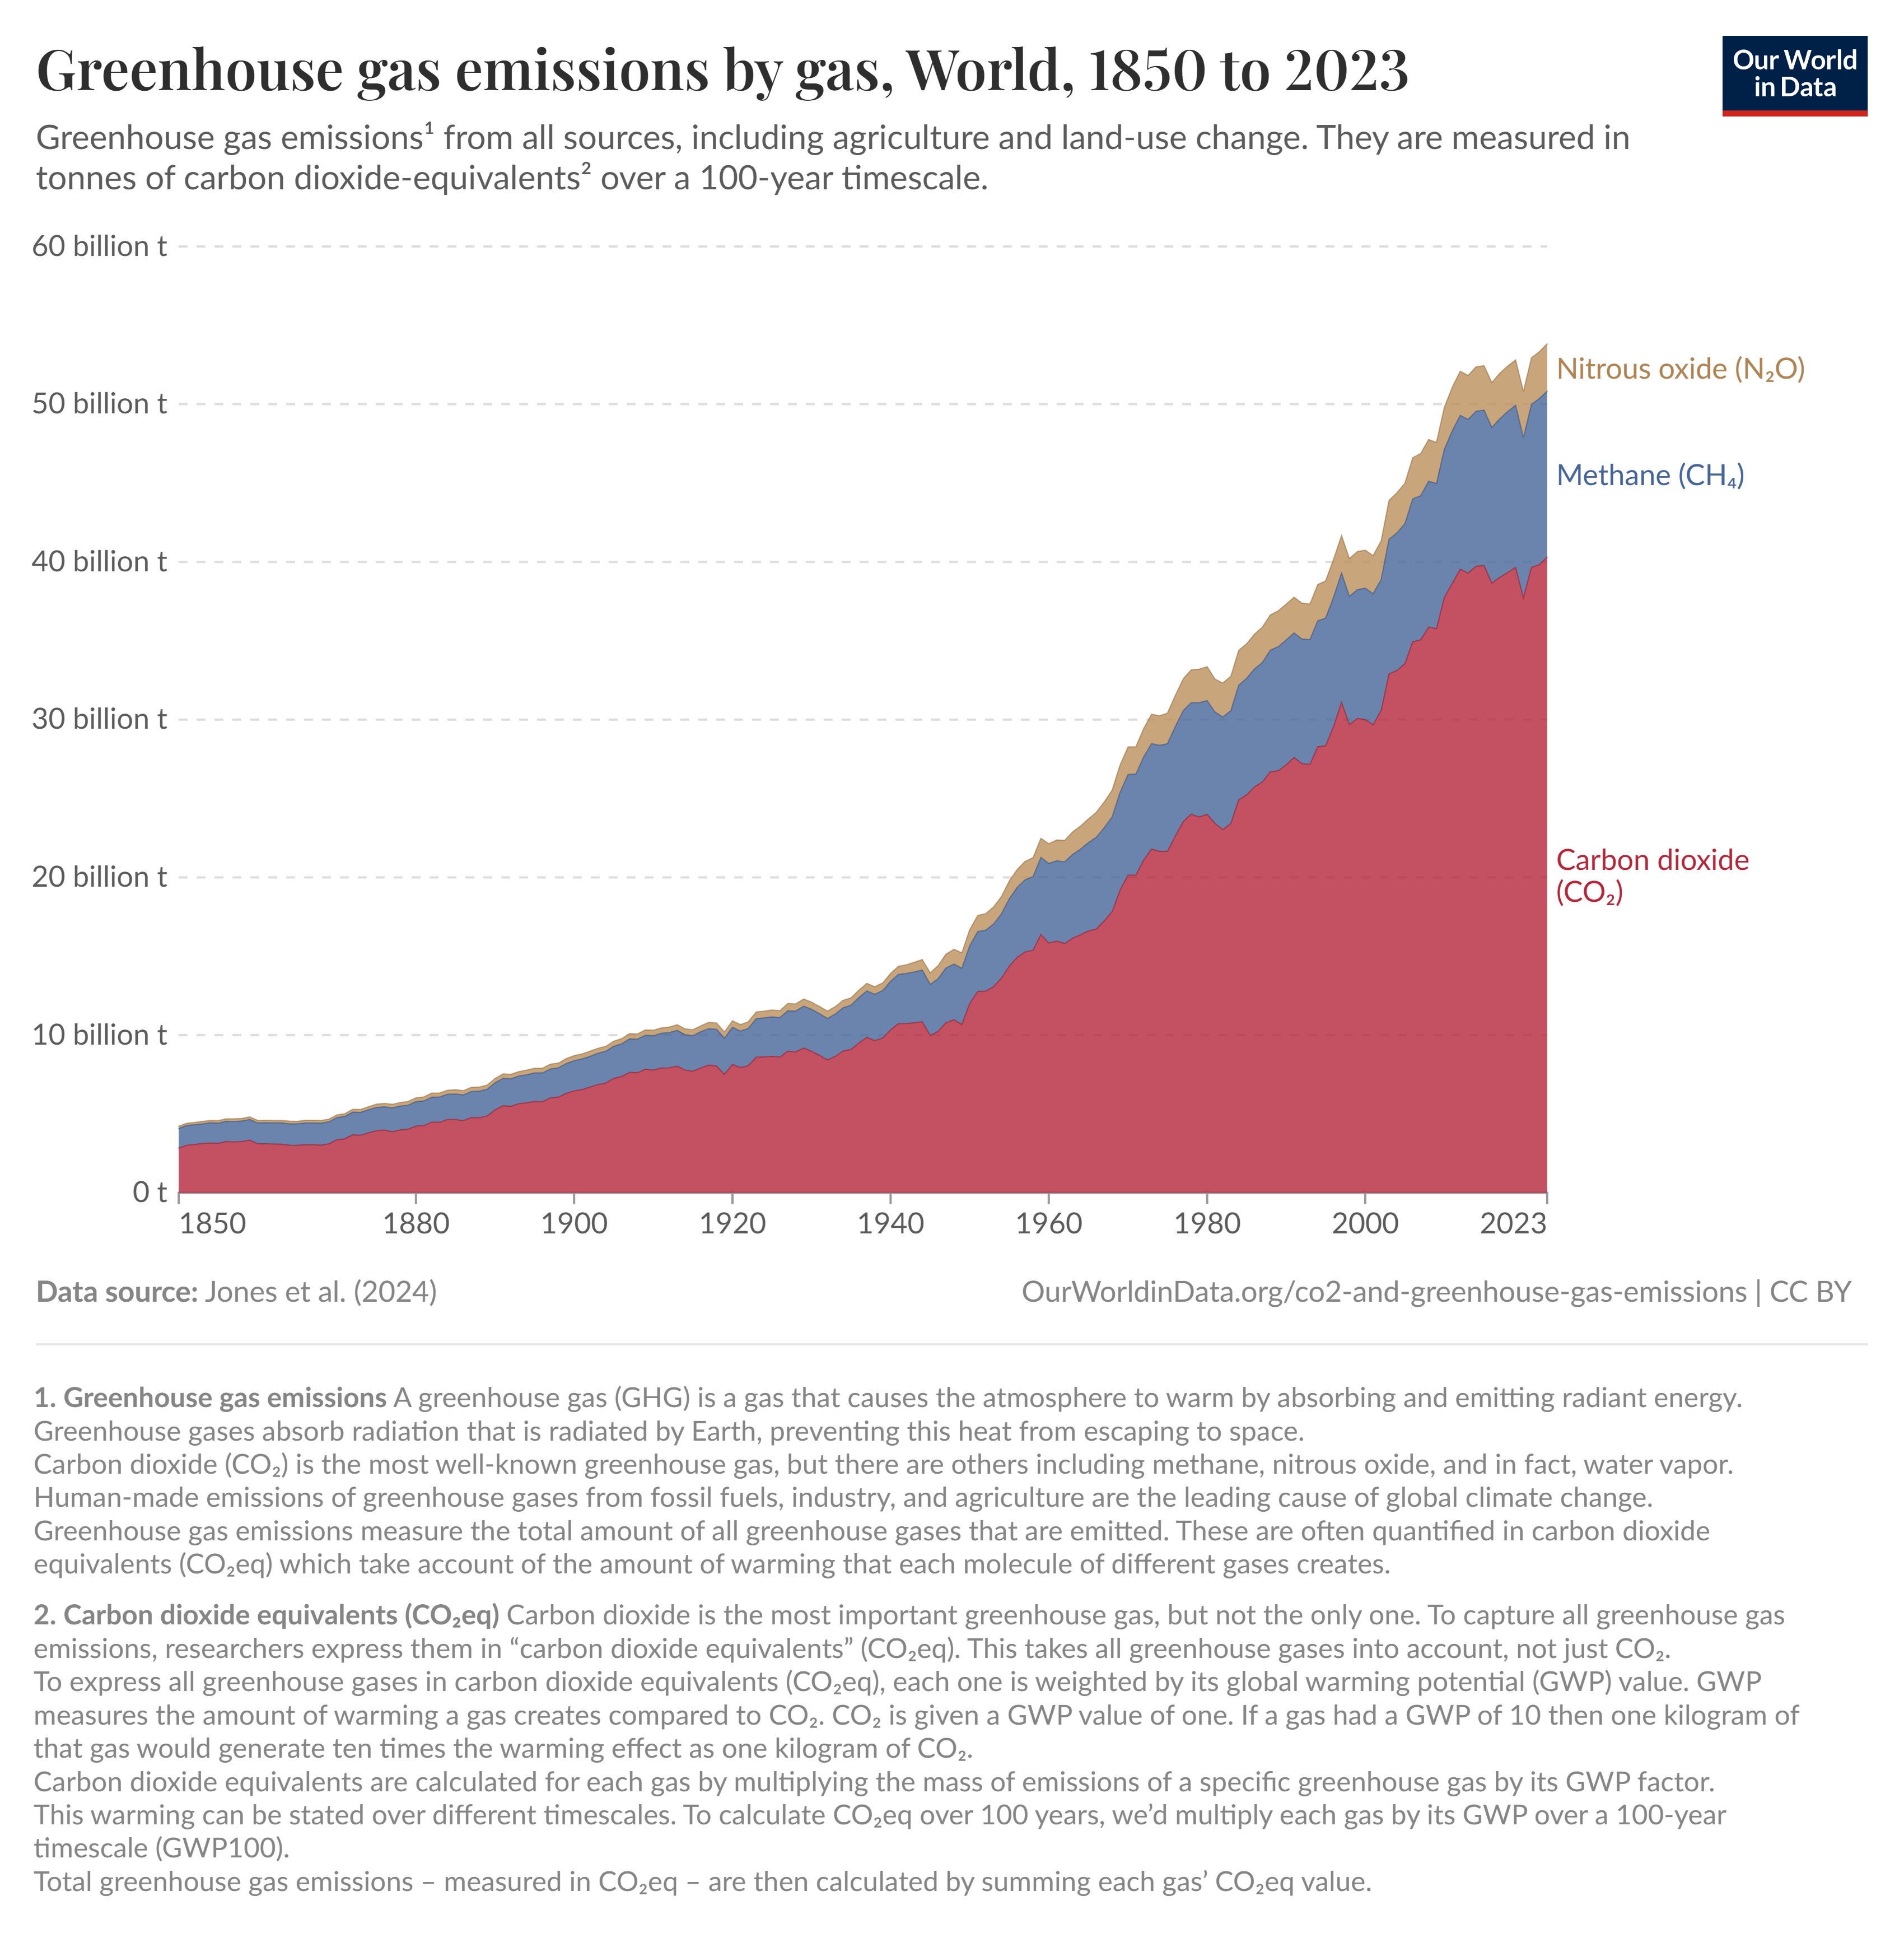
\includegraphics[width=0.7\linewidth]{images/ghg-emissions-by-gas.png}\newline%

%TCIMACRO{\TeXButton{Transition: Box Out}{\transboxout}}%
%BeginExpansion
\transboxout
%EndExpansion%
%TCIMACRO{\TeXButton{EndFrame}{\end{frame}}}%
%BeginExpansion
\end{frame}%
%EndExpansion
%

%TCIMACRO{\TeXButton{BeginFrame}{\begin{frame}}}%
%BeginExpansion
\begin{frame}%
%EndExpansion
%

%TCIMACRO{\QTR{frametitle}{Emissions: GHG\ sources}}%
%BeginExpansion
\frametitle{Emissions: GHG\ sources}%
%EndExpansion


\centering
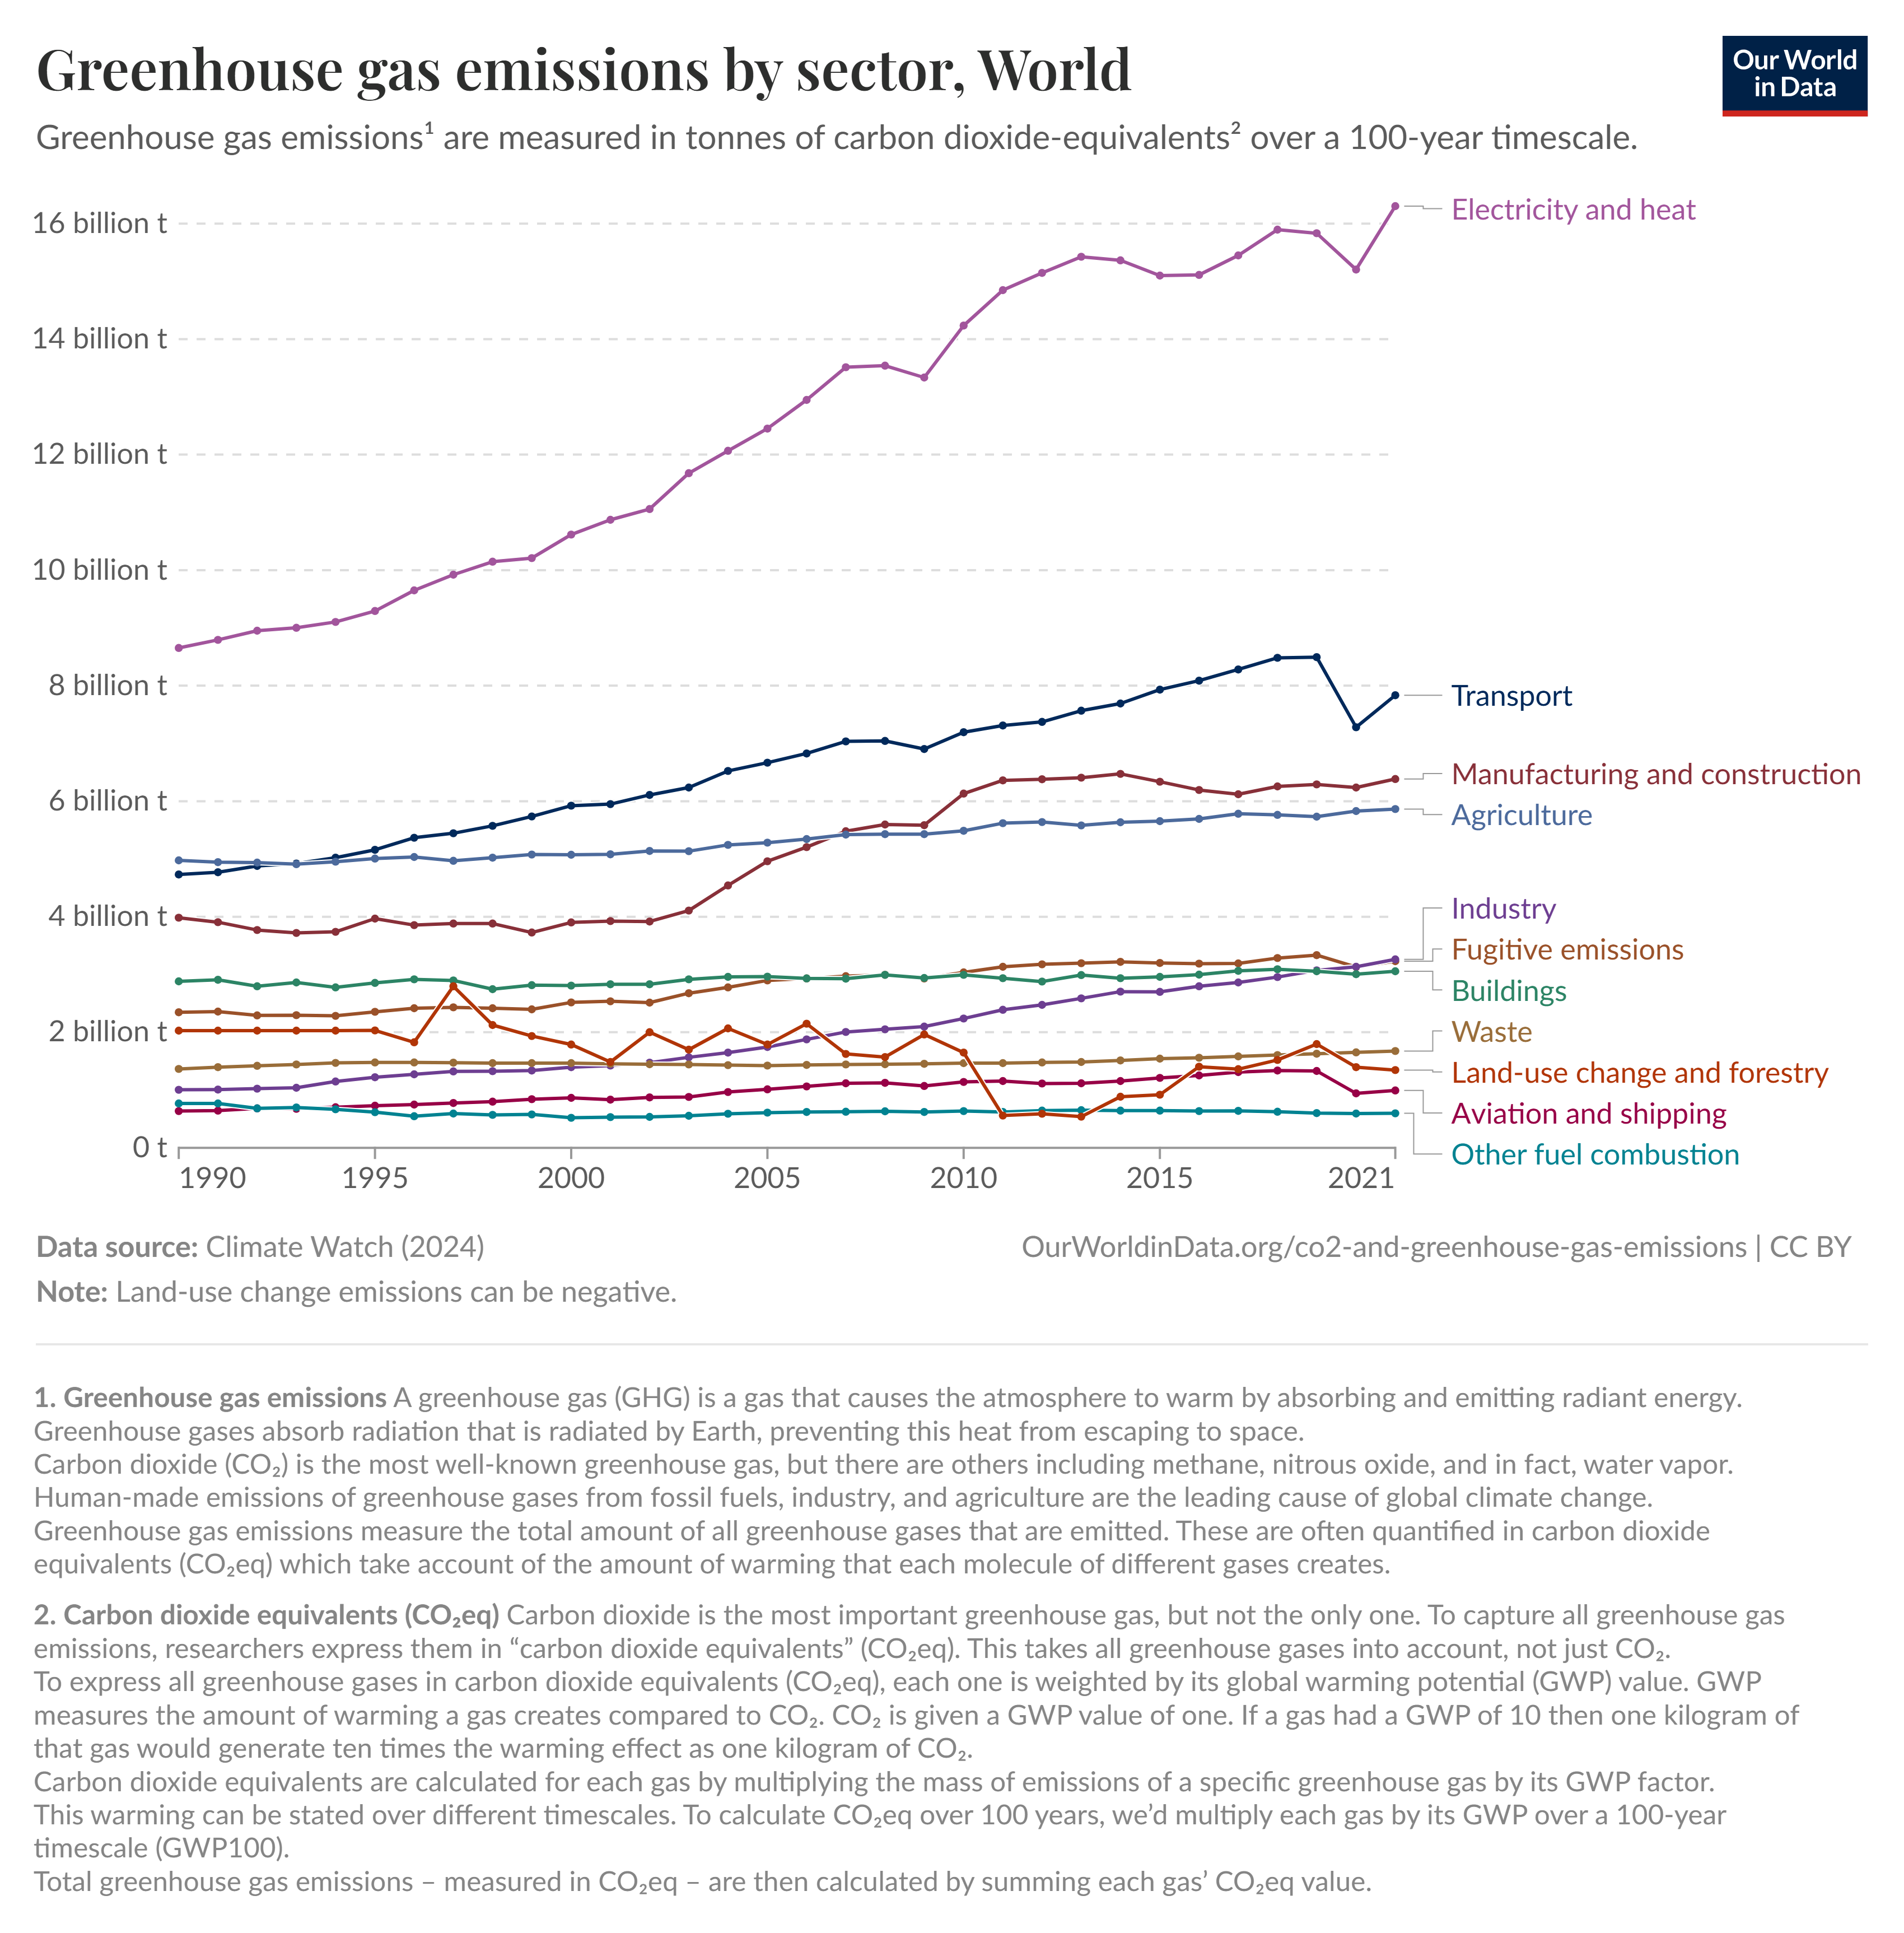
\includegraphics[width=0.7\linewidth]{images/ghg-emissions-by-sector.png}\newline%
%

%TCIMACRO{\TeXButton{Transition: Box Out}{\transboxout}}%
%BeginExpansion
\transboxout
%EndExpansion%
%TCIMACRO{\TeXButton{EndFrame}{\end{frame}}}%
%BeginExpansion
\end{frame}%
%EndExpansion
%

%TCIMACRO{\TeXButton{BeginFrame}{\begin{frame}}}%
%BeginExpansion
\begin{frame}%
%EndExpansion
%

%TCIMACRO{\QTR{frametitle}{Emissions: Scenarios used in simulations}}%
%BeginExpansion
\frametitle{Emissions: Scenarios used in simulations}%
%EndExpansion


\begin{itemize}
\item \textbf{Historical:} observed emissions up to 2020 (e.g.\ OWID data).

\item \textbf{Future:} socio-economic pathways (SSP1--SSP5) used by the IPCC.
\end{itemize}

\vspace{1em} \centering
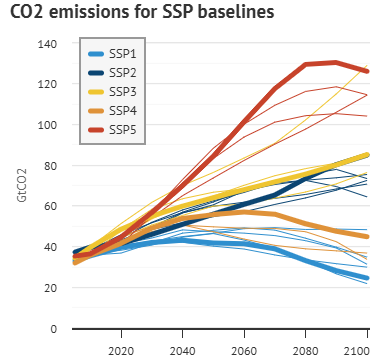
\includegraphics[width=0.25\linewidth]{images/CO2SSP.png}\newline%
\vspace{0.5em} {\footnotesize {Forecasted CO$_{2}$ emissions under SSP
baselines: highlighting the uncertainty from socio-economic pathways.}}%

%TCIMACRO{\TeXButton{Transition: Box Out}{\transboxout}}%
%BeginExpansion
\transboxout
%EndExpansion%
%TCIMACRO{\TeXButton{EndFrame}{\end{frame}}}%
%BeginExpansion
\end{frame}%
%EndExpansion
%

%TCIMACRO{\TeXButton{ENDIF}{\fi}}%
%BeginExpansion
\fi
%EndExpansion
%

%TCIMACRO{\TeXButton{BeginFrame}{\begin{frame}}}%
%BeginExpansion
\begin{frame}%
%EndExpansion
%

%TCIMACRO{\QTR{frametitle}{Emissions: wrap-up}}%
%BeginExpansion
\frametitle{Emissions: wrap-up}%
%EndExpansion


To summarize this section, you only need to remember:

\begin{itemize}
\item In principle, models can take three distinct exogenous inputs:
\[
\{E_{t}^{CO_{2}}\}_{t\geq0},\quad\{E_{t}^{CH_{4}}\}_{t\geq0},\quad
\{E_{t}^{N_{2}O}\}_{t\geq0}.
\]


\item In simplified reduced-form models, only CO$_{2}$ emissions are modeled
explicitly; CH$_{4}$ and N$_{2}$O are often represented by an additional
exogenous forcing term.
\end{itemize}

%

%TCIMACRO{\TeXButton{Transition: Box Out}{\transboxout}}%
%BeginExpansion
\transboxout
%EndExpansion%
%TCIMACRO{\TeXButton{EndFrame}{\end{frame}}}%
%BeginExpansion
\end{frame}%
%EndExpansion


\section{Concentrations}%

%TCIMACRO{\TeXButton{BeginFrame}{\begin{frame}}}%
%BeginExpansion
\begin{frame}%
%EndExpansion
%

%TCIMACRO{\QTR{frametitle}{Concentrations: from to emissions to concetration}}%
%BeginExpansion
\frametitle{Concentrations: from to emissions to concetration}%
%EndExpansion
%

\[
\lbrack\text{Emissions (flows)}]\rightarrow\lbrack\text{%
%TCIMACRO{\TeXButton{red}{\color{red}}}%
%BeginExpansion
\color{red}%
%EndExpansion
\textsf{Atmospheric Concentration }(stock)%
%TCIMACRO{\TeXButton{black}{\color{black}}}%
%BeginExpansion
\color{black}%
%EndExpansion
}]\rightarrow\ldots
\]
From emissions (\textsf{flows}) to concentrations (\textsf{stocks}):

\begin{itemize}
\item Climate does not react directly to annual emissions, but to the
\textbf{cumulative stock of gases} in the atmosphere.

\item Emissions are measured in flows (e.g. GtC/yr).

\item Once emitted, gases accumulate in the atmosphere.

\item What matters for climate forcing is the concentration (ppm or ppb).
\end{itemize}

%

%TCIMACRO{\TeXButton{Transition: Box Out}{\transboxout}}%
%BeginExpansion
\transboxout
%EndExpansion%
%TCIMACRO{\TeXButton{EndFrame}{\end{frame}}}%
%BeginExpansion
\end{frame}%
%EndExpansion
%

%TCIMACRO{\TeXButton{BeginFrame}{\begin{frame}}}%
%BeginExpansion
\begin{frame}%
%EndExpansion
%

%TCIMACRO{\QTR{frametitle}{Cnocentrations: Atmospheric concentrations}}%
%BeginExpansion
\frametitle{Cnocentrations: Atmospheric concentrations}%
%EndExpansion


\centering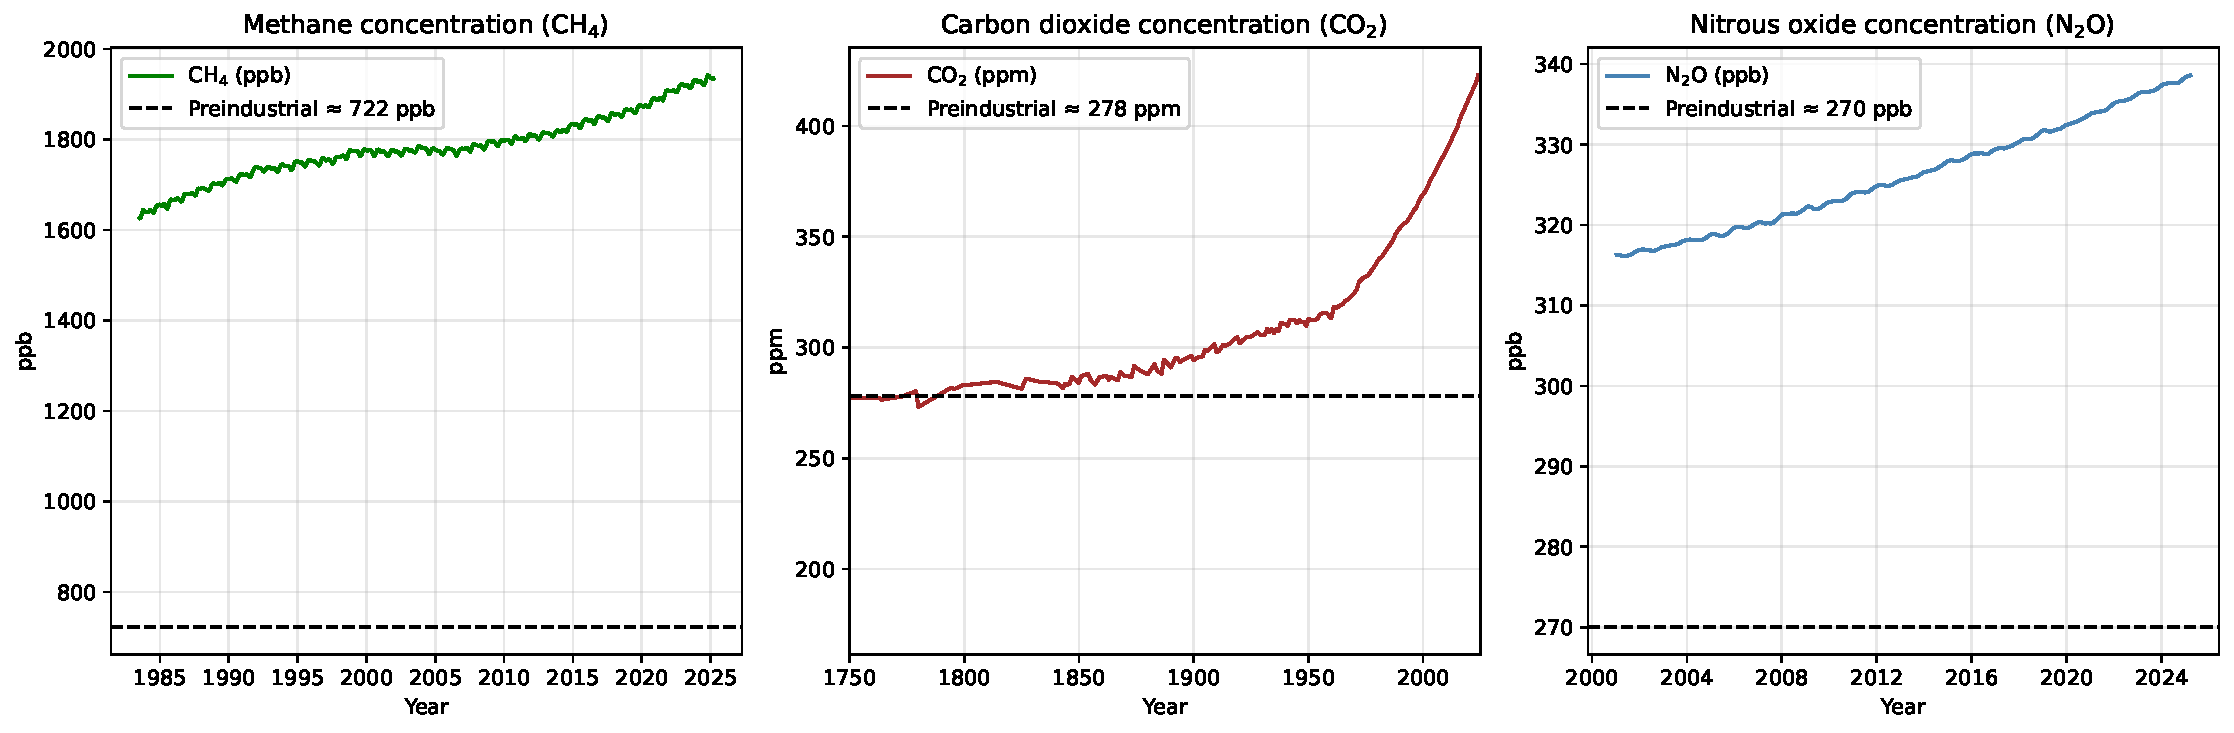
\includegraphics[width=1\linewidth]{images/concentrations.pdf}\newline%
%

%TCIMACRO{\TeXButton{Transition: Box Out}{\transboxout}}%
%BeginExpansion
\transboxout
%EndExpansion%
%TCIMACRO{\TeXButton{EndFrame}{\end{frame}}}%
%BeginExpansion
\end{frame}%
%EndExpansion
%

%TCIMACRO{\TeXButton{BeginFrame}{\begin{frame}}}%
%BeginExpansion
\begin{frame}
\frametitle{Concentrations: ODE and discrete periods}
\small
Let $s$ be calendar time, $s_t=s_0+t\Delta$, and $t$ the period index.
The next observation is $t+1$, separated by $\Delta$ years.
\[
\frac{d\mathbf M_g(s)}{ds}
=\mathbf A_g\big(\mathbf M_g(s)-\overline{\mathbf M}_g\big)
+\mathbf b_g E^g(s).
\]
\[
\boxed{\mathbf M_{g,t+1}=\mathbf M_{g,t}
+\Delta\mathbf A_g\big(\mathbf M_{g,t}-\overline{\mathbf M}_g\big)
+\Delta\mathbf b_g E^g_t.}
\]
\begin{itemize}
\item $\overline{\mathbf M}_g$: natural equilibrium; $\mathbf M_{g,0}$:
given initial state. They need not coincide.
\item $\mathbf A_g$: annual transfer/removal rates; $\mathbf b_g$:
injection and unit conversion. $E^g_t$ is an annual emissions rate.
\item Forward Euler: evaluate all terms at the old state, then multiply
rates by $\Delta$. Zero input leaves the reference state stationary.
\end{itemize}
\transboxout
\end{frame}
%EndExpansion
%

%TCIMACRO{\TeXButton{BeginFrame}{\begin{frame}}}%
%BeginExpansion
\begin{frame}%
%EndExpansion
%

%TCIMACRO{\QTR{frametitle}{Cnocentrations: Some precisions}}%
%BeginExpansion
\frametitle{Cnocentrations: Some precisions}%
%EndExpansion


\medskip\textbf{Modeling choice.} The number of boxes $n_{g}$ determines precision:

\begin{itemize}
\item $n_{g}=1$: a single decay process (e.g.\ CH$_{4}$, N$_{2}$O).

\item $n_{g}=2$--$3$: separates atmosphere, fast reservoirs (biosphere/upper
ocean), and slow reservoirs (deep ocean) for CO$_{2}$.

\item Larger $n_{g}$: more realistic sequestration processes (soil carbon,
permafrost, multiple ocean layers) at the cost of extra parameters.
\vspace{2ex}
\end{itemize}

\textbf{Conservation: }

\begin{itemize}
\item the system is physical, so total mass is conserved: transfers occur
\textit{between} boxes, with no loss outside the system (except for explicitly
modelled sinks).
\end{itemize}

%

%TCIMACRO{\TeXButton{Transition: Box Out}{\transboxout}}%
%BeginExpansion
\transboxout
%EndExpansion%
%TCIMACRO{\TeXButton{EndFrame}{\end{frame}}}%
%BeginExpansion
\end{frame}%
%EndExpansion
%

%TCIMACRO{\TeXButton{BeginFrame}{\begin{frame}}}%
%BeginExpansion
\begin{frame}
\frametitle{Concentrations: the three-box carbon cycle}
\small
\[
\mathbf M_t=(M_{AT,t},M_{UP,t},M_{LO,t})^\top,
\]
\[
\mathbf M_{t+1}=\overline{\mathbf M}
+\boldsymbol\Phi(\mathbf M_t-\overline{\mathbf M})
+\Delta\boldsymbol\Xi E^{CO_2}_t.
\]
\[
\boldsymbol\Phi=I+\Delta\mathbf A,\qquad
\boldsymbol\Phi\overline{\mathbf M}=\overline{\mathbf M},\qquad
\boldsymbol\Xi=(3/11,0,0)^\top.
\]
\begin{itemize}
\item Stocks are in GtC; emissions are in GtCO$_2$/year.
Only the atmosphere receives emissions directly.
\item The equilibrium identity gives the equivalent level equation
$\mathbf M_{t+1}=\boldsymbol\Phi\mathbf M_t+\Delta\boldsymbol\Xi E^{CO_2}_t$.
\item Column sums of $\boldsymbol\Phi$ equal one: internal transfers
conserve total carbon, which rises by $\Delta(3/11)E^{CO_2}_t$.
\item Reference stocks: $\overline{\mathbf M}=(588,360,1720)^\top$;
default 2015 state: $\mathbf M_0=(851,460,1740)^\top$.
\end{itemize}
\transboxout
\end{frame}
%EndExpansion
%

%TCIMACRO{\TeXButton{BeginFrame}{\begin{frame}}}%
%BeginExpansion
\begin{frame}
\frametitle{Concentrations: methane decay relative to a baseline}
\small
\[
\boxed{M^{CH_4}_{t+1}=\overline M^{CH_4}
+(1-\Delta\delta_{CH_4})(M^{CH_4}_t-\overline M^{CH_4})
+\Delta\kappa_{CH_4}E^{CH_4}_t.}
\]
\begin{itemize}
\item $\overline M^{CH_4}=722$ ppb is the preindustrial reference.
The default initial concentration is $M^{CH_4}_0=1860$ ppb.
\item Only the \emph{excess above the reference} decays. Without additional
emissions, methane returns towards 722 ppb, not zero.
\item Course calibration: $\delta_{CH_4}=1/9$ year$^{-1}$,
so the characteristic lifetime is 9 years.
\item For emissions in MtCH$_4$/year, $\kappa_{CH_4}=1/2.78$ ppb/MtCH$_4$.
The notebook converts inputs to ppb/year before calling the module;
the module therefore uses $\kappa_{CH_4}=1$ on that converted input.
\end{itemize}
\transboxout
\end{frame}
%EndExpansion


\section{Radiative Forcing}%

%TCIMACRO{\TeXButton{BeginFrame}{\begin{frame}}}%
%BeginExpansion
\begin{frame}%
%EndExpansion
%

%TCIMACRO{\QTR{frametitle}{Forcing: Definition}}%
%BeginExpansion
\frametitle{Forcing: Definition}%
%EndExpansion%
\[
\lbrack\text{\textsf{Emissions} (flows)}]\rightarrow\lbrack
\text{\textsf{Concentration} (stock)}]\rightarrow\lbrack\text{%
%TCIMACRO{\TeXButton{red}{\color{red}}}%
%BeginExpansion
\color{red}%
%EndExpansion
\textsf{Forcing} (flow)%
%TCIMACRO{\TeXButton{black}{\color{black}}}%
%BeginExpansion
\color{black}%
%EndExpansion
}]\rightarrow\ldots
\]


\textbf{Key idea.} Radiative forcing is the \emph{side effect of rising
concentrations}: it increases the thickness of the atmospheric ``blanket''
that traps heat. \medskip

\begin{itemize}
\item \textbf{Baseline:} in the preindustrial climate, incoming solar
$\approx$ outgoing infrared (energy balance).

\item \textbf{Forcing:} any perturbation that shifts this balance.

\begin{itemize}
\item Positive forcing $\;\Rightarrow\;$ warming (extra blanket from GHGs).

\item Negative forcing $\;\Rightarrow\;$ cooling (reflective aerosols,
volcanic dust).
\end{itemize}

\item \textbf{Units.} Watts per square meter (W/m$^{2}$).
\end{itemize}

%

%TCIMACRO{\TeXButton{Transition: Box Out}{\transboxout}}%
%BeginExpansion
\transboxout
%EndExpansion%
%TCIMACRO{\TeXButton{EndFrame}{\end{frame}}}%
%BeginExpansion
\end{frame}%
%EndExpansion
%

%TCIMACRO{\TeXButton{BeginFrame}{\begin{frame}}}%
%BeginExpansion
\begin{frame}
\frametitle{Forcing: reference levels and timing}
\small
Forcing is an energy imbalance relative to the reference climate,
not an additional state variable.
\[
F_t=\sum_{g\in\{CO_2,CH_4,N_2O\}}F^g_t+F^{\mathrm{ex}}_t,
\qquad
F^g_t=f_g(M^g_{AT,t-1})-f_g(\overline M^g_{AT}).
\]
\begin{itemize}
\item $\overline M^g_{AT}$ is the preindustrial level, not the initial
concentration at the start of a modern simulation.
\item Code convention: $F_t$ acts during the transition from $t-1$ to $t$
and is computed from the \emph{old} concentrations $M^g_{AT,t-1}$.
\item Equivalently, $F_{t+1}=\sum_g[f_g(M^g_{AT,t})-
f_g(\overline M^g_{AT})]+F^{\mathrm{ex}}_{t+1}$.
\item The course module includes CO$_2$ and CH$_4$ only; no overlap
correction, explicit N$_2$O or other external forcing is included.
\end{itemize}
\transboxout
\end{frame}
%EndExpansion
%

%TCIMACRO{\TeXButton{BeginFrame}{\begin{frame}}}%
%BeginExpansion
\begin{frame}%
%EndExpansion
%

%TCIMACRO{\QTR{frametitle}{Forcing: Some illustration}}%
%BeginExpansion
\frametitle{Forcing: Some illustration}%
%EndExpansion


\begin{center}
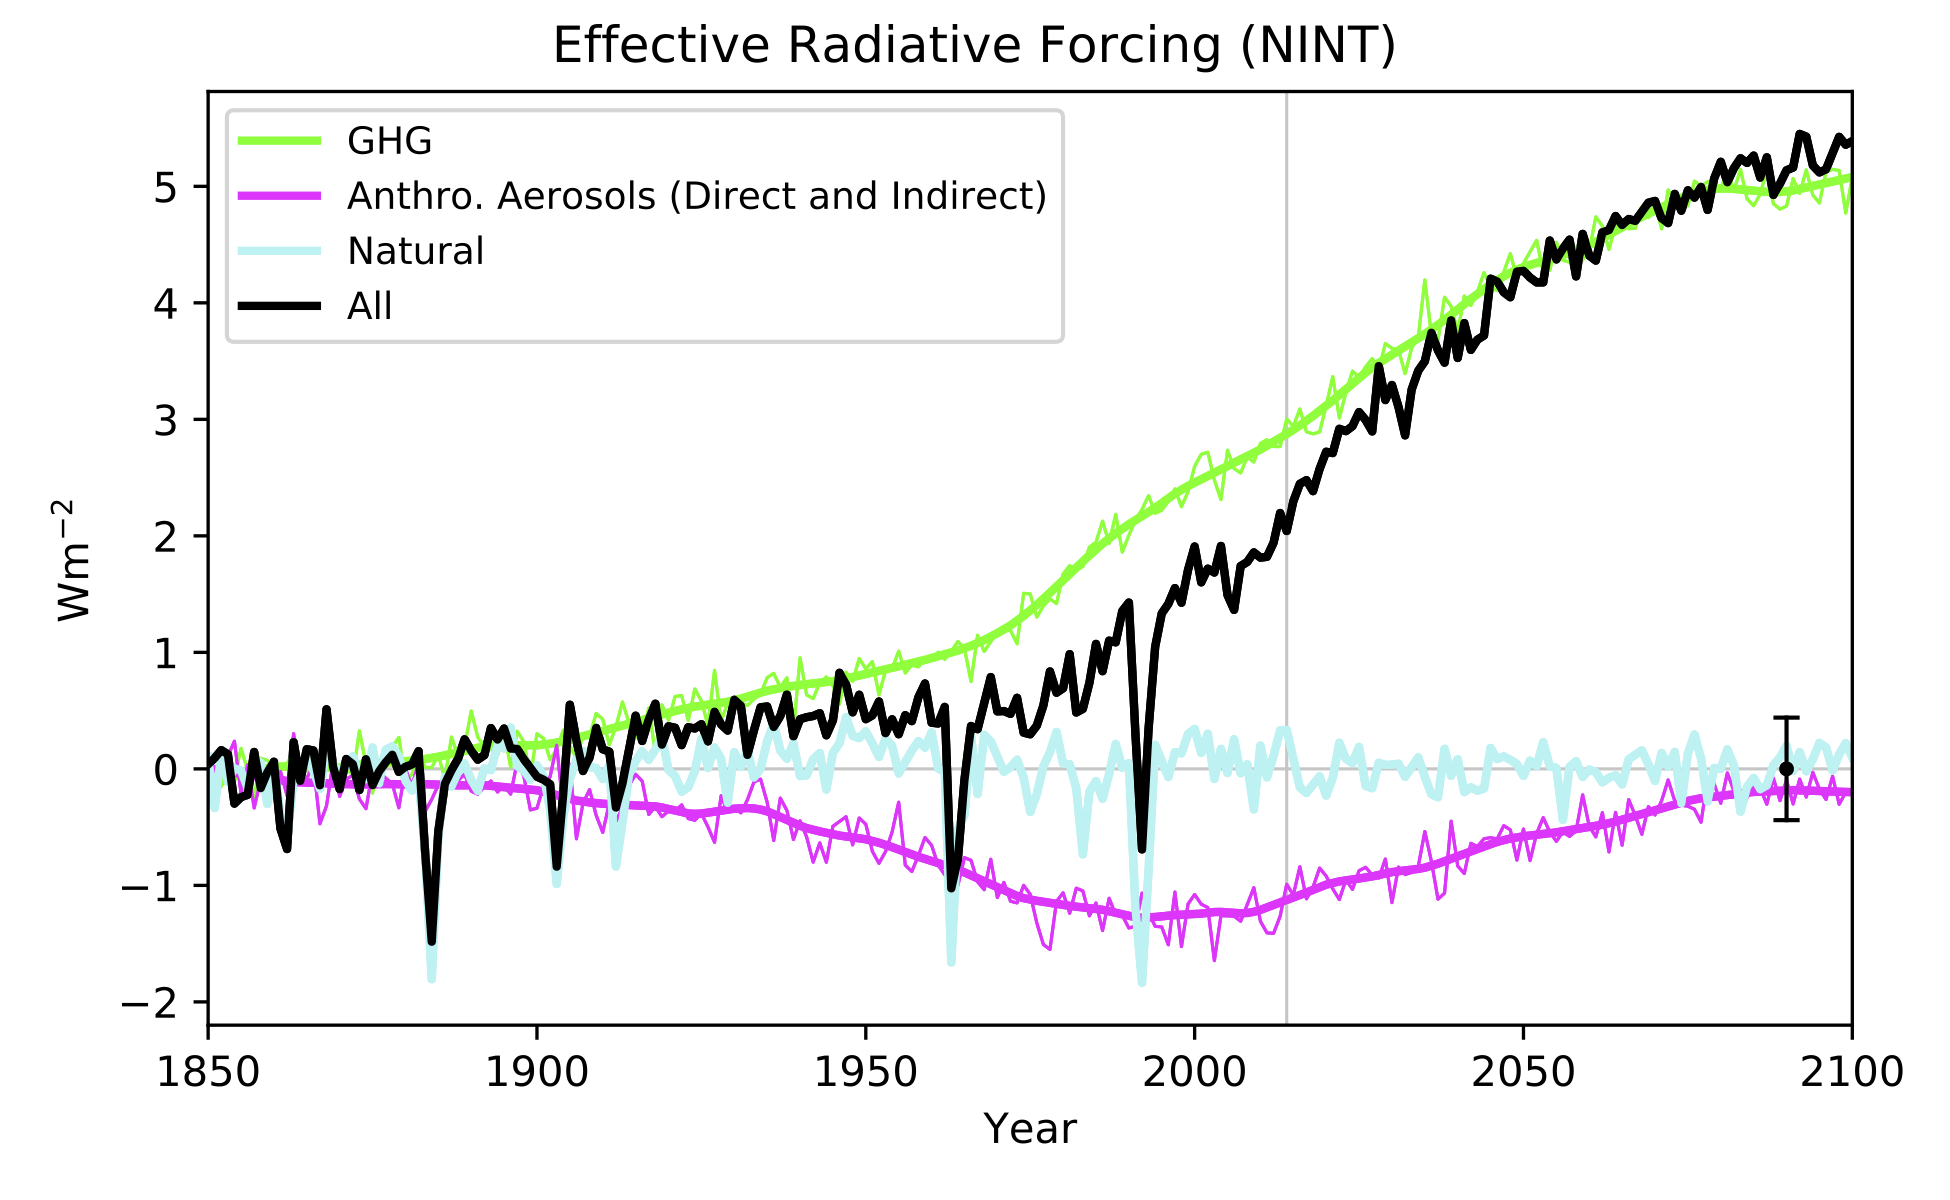
\includegraphics[width=0.5\textwidth]{images/ERF_glb_historical_E2-1_f2.png}
\end{center}

\begin{itemize}
\item \textbf{Pink line:} Anthropogenic aerosols $\;\Rightarrow$
\emph{negative forcing}.

e.g.\ sulfate aerosols (from burning coal and oil- $SO_{2}$ emissions), very
reflective: scatter sunlight back to space, short lifetime (days-weeks).

\item \textbf{Cyan line:} Natural forcings (solar variability, volcanic eruptions).
\end{itemize}

%

%TCIMACRO{\TeXButton{Transition: Box Out}{\transboxout}}%
%BeginExpansion
\transboxout
%EndExpansion%
%TCIMACRO{\TeXButton{EndFrame}{\end{frame}}}%
%BeginExpansion
\end{frame}%
%EndExpansion
%

%TCIMACRO{\TeXButton{BeginFrame}{\begin{frame}}}%
%BeginExpansion
\begin{frame}
\frametitle{Forcing: carbon dioxide}
\begin{block}{Logarithmic forcing relative to preindustrial carbon}
\[
F^{CO_2}_t=F_{2\times CO_2}
\frac{\ln\!\left(M^{CO_2}_{AT,t-1}/\overline M^{CO_2}_{AT}\right)}{\ln 2}.
\]
\end{block}
\begin{itemize}
\item Use the same units in numerator and denominator.
In the module, carbon is in GtC and $\overline M^{CO_2}_{AT}=588$ GtC.
\item Course calibration: $F_{2\times CO_2}=3.3613$ W/m$^2$.
At twice the reference stock, the forcing is exactly $F_{2\times CO_2}$.
\item With the default initial stock $M^{CO_2}_{AT,0}=851$ GtC,
the first-interval CO$_2$ forcing is
\[
F^{CO_2}_1=3.3613\,\frac{\ln(851/588)}{\ln 2}
\simeq 1.79\;\mathrm{W/m^2}.
\]
\end{itemize}
\transboxout
\end{frame}
%EndExpansion
%

%TCIMACRO{\TeXButton{BeginFrame}{\begin{frame}}}%
%BeginExpansion
\begin{frame}
\frametitle{Forcing: methane}
\begin{block}{Square-root forcing relative to preindustrial methane}
\[
F^{CH_4}_t=\alpha_{CH_4}
\left(\sqrt{M^{CH_4}_{t-1}}-\sqrt{\overline M^{CH_4}}\right).
\]
\end{block}
\begin{itemize}
\item Reference: $\overline M^{CH_4}=722$ ppb;
default initial concentration: $M^{CH_4}_0=1860$ ppb.
\item $\alpha_{CH_4}=0.036\;\mathrm{W/m^2}/\sqrt{\mathrm{ppb}}$.
The forcing vanishes at the reference, not at the modern initial state.
\item First-interval methane forcing:
\[
F^{CH_4}_1=0.036\left(\sqrt{1860}-\sqrt{722}\right)
\simeq 0.59\;\mathrm{W/m^2}.
\]
\end{itemize}
\transboxout
\end{frame}
%EndExpansion


\section{Temperatures (output)}%

%TCIMACRO{\TeXButton{BeginFrame}{\begin{frame}}}%
%BeginExpansion
\begin{frame}%
%EndExpansion
%

%TCIMACRO{\QTR{frametitle}{Temperatures: Dynamics}}%
%BeginExpansion
\frametitle{Temperatures: Dynamics}%
%EndExpansion
%

\[
\lbrack\text{\textsf{Emissions} (flows)}]\rightarrow\lbrack
\text{\textsf{Concentration} (stock)}]\rightarrow\lbrack\text{\textsf{Forcing}
(flow)}]\rightarrow\lbrack\text{%
%TCIMACRO{\TeXButton{red}{\color{red}}}%
%BeginExpansion
\color{red}%
%EndExpansion
\textsf{Temperature} (stock)%
%TCIMACRO{\TeXButton{black}{\color{black}}}%
%BeginExpansion
\color{black}%
%EndExpansion
}]
\]


\medskip

\begin{itemize}
\item \textbf{Key point:} Radiative forcing $\neq$ instantaneous warming.

Temperatures behave as a \emph{state variable}: they accumulate the effect of
past forcings, with strong inertia.

\item \textbf{Sources of inertia:}

\begin{itemize}
\item The ocean absorbs most of the excess heat, releasing it slowly.

\item Ice sheets and cryosphere respond on multi-decadal to millennial scales.

\item Feedbacks (clouds, carbon cycle) operate with delays.
\end{itemize}

\item \textbf{Illustration: }Even if CO$_{2}$ concentrations stabilized today,
global temperatures would still rise for decades (\textquotedblleft committed
warming\textquotedblright).
\end{itemize}

%

%TCIMACRO{\TeXButton{Transition: Box Out}{\transboxout}}%
%BeginExpansion
\transboxout
%EndExpansion%
%TCIMACRO{\TeXButton{EndFrame}{\end{frame}}}%
%BeginExpansion
\end{frame}%
%EndExpansion
%

%TCIMACRO{\TeXButton{BeginFrame}{\begin{frame}}}%
%BeginExpansion
\begin{frame}
\frametitle{Temperatures: ODE and explicit time stepping}
\small
Temperature anomalies are measured relative to the reference climate,
so $\overline{\mathbf T}=\mathbf 0$ (not necessarily $\mathbf T_0$).
\[
\frac{d\mathbf T(s)}{ds}
=\mathbf A_T\big(\mathbf T(s)-\overline{\mathbf T}\big)
+\mathbf B_T F(s).
\]
\[
\boxed{\mathbf T_t=\mathbf T_{t-1}
+\Delta\Big[\mathbf A_T(\mathbf T_{t-1}-\overline{\mathbf T})
+\mathbf B_T F_t\Big].}
\]
\begin{itemize}
\item All temperature terms on the right use $t-1$;
$F_t$ is computed from the gas stocks at $t-1$.
\item Equivalently, advance from $\mathbf T_t$ to $\mathbf T_{t+1}$
using $F_{t+1}$. The index advances by one, not by $\Delta$.
\item The reference is already subtracted in an anomaly.
Initial anomalies are given: zero for the preindustrial experiment,
$(0.85,0.007)^\top$ in the default 2015 calibration.
\end{itemize}
\transboxout
\end{frame}
%EndExpansion
%

%TCIMACRO{\TeXButton{BeginFrame}{\begin{frame}}}%
%BeginExpansion
\begin{frame}
\frametitle{Temperatures: the two-box model}
\small
\[
\begin{aligned}
T^{AT}_t &= T^{AT}_{t-1}+\Delta c_1\Big[
F_t-\lambda T^{AT}_{t-1}
-c_3(T^{AT}_{t-1}-T^{LO}_{t-1})\Big],\\[0.5em]
T^{LO}_t &= T^{LO}_{t-1}
+\Delta c_4(T^{AT}_{t-1}-T^{LO}_{t-1}),
\qquad \lambda=\frac{F_{2\times CO_2}}{T_{2\times CO_2}}.
\end{aligned}
\]
\begin{itemize}
\item $T^{AT},T^{LO}$ are anomalies relative to the preindustrial reference;
there is no additional subtraction of the modern initial temperature.
\item $c_1F_t$ heats the surface; $c_1\lambda T^{AT}_{t-1}$ is radiative
restoration; the difference $T^{AT}_{t-1}-T^{LO}_{t-1}$ drives ocean heat uptake.
\item $F_t=F^{CO_2}_t+F^{CH_4}_t$ uses gas stocks at $t-1$.
The deep ocean also uses the old surface temperature, not $T^{AT}_t$.
\item Give both initial anomalies at the chosen start date.
Only a preindustrial initial state has $T^{AT}_0=T^{LO}_0=0$.
\end{itemize}
\transboxout
\end{frame}
%EndExpansion
%

%TCIMACRO{\TeXButton{BeginFrame}{\begin{frame}}}%
%BeginExpansion
\begin{frame}
\frametitle{Temperatures: equilibrium under doubled CO$_2$}
\small
Hold atmospheric CO$_2$ at twice its reference level and set all
other forcing contributions to zero.
\[
M^{CO_2}_{AT}=2\overline M^{CO_2}_{AT}
\quad\Longrightarrow\quad
F=F_{2\times CO_2}=3.3613\;\mathrm{W/m^2}.
\]
\[
\begin{aligned}
T^{AT}_t &= T^{AT}_{t-1}+\Delta c_1\Big[
F_{2\times CO_2}-\lambda T^{AT}_{t-1}
-c_3(T^{AT}_{t-1}-T^{LO}_{t-1})\Big],\\
T^{LO}_t &= T^{LO}_{t-1}+\Delta c_4(T^{AT}_{t-1}-T^{LO}_{t-1}).
\end{aligned}
\]
At equilibrium both temperature changes vanish:
\[
T^{AT,*}=T^{LO,*}=\frac{F_{2\times CO_2}}{\lambda}
=T_{2\times CO_2}=3.1\,{}^\circ\mathrm C.
\]
This is the long-run anomaly, not an immediate jump in temperature.
The experiment holds concentration fixed; it is not a zero-emissions run.
\transboxout
\end{frame}
%EndExpansion
%

%TCIMACRO{\TeXButton{BeginFrame}{\begin{frame}}}%
%BeginExpansion
\begin{frame}%
%EndExpansion
%

%TCIMACRO{\QTR{frametitle}{Temperatures: Human vs. Natural Forcings}}%
%BeginExpansion
\frametitle{Temperatures: Human vs. Natural Forcings}%
%EndExpansion


\begin{center}
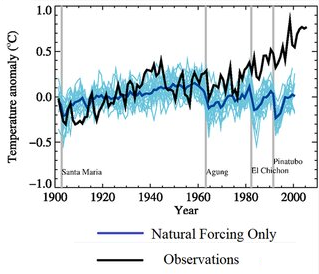
\includegraphics[width=0.5\textwidth]{images/The-ensembles-between-the-global-observed-temperature-anomalies-and-the-simulated-ones-by_W640.png}
\end{center}

%

%TCIMACRO{\TeXButton{Transition: Box Out}{\transboxout}}%
%BeginExpansion
\transboxout
%EndExpansion%
%TCIMACRO{\TeXButton{EndFrame}{\end{frame}}}%
%BeginExpansion
\end{frame}%
%EndExpansion
%

%TCIMACRO{\TeXButton{BeginFrame}{\begin{frame}}}%
%BeginExpansion
\begin{frame}
\frametitle{To wrap up: stocks, forcing and temperature}
\small
Consider an instantaneous addition of 1 GtC to the atmosphere, starting
from the preindustrial reference $\overline M_{AT}=588$ GtC.
\[
M_{AT}:588\longmapsto589\;\mathrm{GtC},\qquad
\Delta F=3.3613\,\frac{\ln(589/588)}{\ln 2}
\simeq 0.0082\;\mathrm{W/m^2}.
\]
\begin{itemize}
\item Atmospheric carbon changes first; forcing responds to the stock
relative to its reference. Temperature does not jump instantaneously.
\item A real pulse is then redistributed between the three carbon boxes;
its subsequent forcing is not constant.
\item Only if the extra atmospheric stock were \emph{held fixed} would
the long-run temperature change be
\[
\Delta T^*=\frac{\Delta F}{\lambda}\simeq0.0076\,{}^\circ\mathrm C,
\qquad \lambda=3.3613/3.1.
\]
\end{itemize}
\transboxout
\end{frame}
%EndExpansion
%

%TCIMACRO{\TeXButton{BeginFrame}{\begin{frame}}}%
%BeginExpansion
\begin{frame}%
%EndExpansion


\begin{center}
Thank you!

\vspace{5ex}

$gauthier.vermandel@polytechnique.edu$
\end{center}

%

%TCIMACRO{\TeXButton{Transition: Box Out}{\transboxout}}%
%BeginExpansion
\transboxout
%EndExpansion%
%TCIMACRO{\TeXButton{EndFrame}{\end{frame}}}%
%BeginExpansion
\end{frame}%
%EndExpansion

\end{document}
